\documentclass[a4paper]{scrartcl}
\usepackage[round,authoryear]{natbib}
\usepackage{graphicx}
\usepackage{color}
\usepackage{multirow}
\usepackage{amsmath}
\usepackage{epstopdf}

\usepackage{setspace}

\begin{document}
\sffamily
\title{
Seasons of the Red King: Mutualism under ecological fluctuations
}   
\author{Chaitanya S. Gokhale and Arne Traulsen\\
Research Group for Evolutionary Theory,\\
Max-Planck-Institute for Evolutionary Biology,\\
August-Thienemann-Stra{\ss}e 2, 24306 Pl\"{o}n, Germany
}

\date{}    
\maketitle

\onehalfspacing

\begin{abstract}
{
\sffamily
Coevolution of two species is typically thought to favor the evolution of faster evolutionary rates helping a species keep ahead in the Red Queen race,
where `it takes all the running you can do to stay where you are'.
In contrast, if species are in a mutualistic relationship, it was proposed that the Red King effect may act, where it can be beneficial to evolve slower than the mutualistic species.
The Red King hypothesis proposes that the species which evolves slower can gain a larger share of the benefits.
Furthermore interactions between species can naturally be assumed to be nonlinear in fashion, thus amenable to modeling by multiplayer games.
However this complexity actually helps us move seamlessly between the the Red King (mutualism) and the Red Queen (antagonistic) kind of interactions.
Incorporating ecological dynamics 
}
\end{abstract}

\sffamily

In his book `The History of Animals', Aristotle observes
{\em
`When the crocodile yawns, the trochilus flies into his mouth and cleans
his teeth. The trochilus gets his food thereby, and the crocodile
gets ease and comfort; it makes no attempt to injure its little friend,
but, when it wants it to go, it shakes its neck in warning, lest it
should accidentally bite the bird'} \citep{aristotle:350bc}.
The phenomenon described by Aristotle was termed as mutualism in $1873$ by the Belgian zoologist Pierre van Beneden \citep{bronstein:2003bo}.
Mutualistic relationships, interspecific interactions that benefit both species, have been empirically studied for many years \citep{boucher:1985aa,hinton:1951aa,wilson:1983an,bronstein:1994aa,pierce:2002aa,kiers:2003aa,bshary:2003bo} and also a considerable body of theory has been put forth trying to explain the evolution and maintenance of such relationships \citep{poulin:1995aa,doebeli:1998aa,noe:2001aa,johnstone:2002aa,bergstrom:2003jf,hoeksema:2003aa,akcay:2007aa,bshary:2008aa}.
The example described by Aristotle and most other examples of mutualisms lend themselves to the idea of direct reciprocity \citep{trivers:1971hp} and thus can be studied using evolutionary game theory.
The interactions in these models are usually dyadic.
A representative of each species is chosen and the outcome of the interactions between these representatives 
determines the evolutionary dynamics within each of the two species.
However, in many cases interactions between species cannot be reduced to such dyadic encounters \citep{stadler:2008bo}.

For example, in the interaction between ants and aphids or butterfly larvae \citep{pierce:1987aa,holldobler:1990an} many ants tend to these soft bodies creatures, providing them with shelter and protection from predation and parasites in exchange for honeydew, a rich source of food for the ants \citep{hill:1989aa,stadler:2008bo}.
This is not a one to one interaction between a larva and an ant, but rather a one to many interaction from the perspective of the larva.
In this manuscript we focus on this kind of -- possibly -- many to many interactions between two mutualistic species.



To analyze how benefits are shared between the two mutualistic species, we make use of evolutionary game theory.
Since we consider the interaction of two species, we resort to bimatrix games
\citep{weibull:1995hp,hofbauer:1996mm,hofbauer:1998mm}.
We consider a situation where benefits can be split in different ways.
Note that the two strategies to generate the benefits and even the benefits themselves
could be completely different, as in the example discussed above. 
If the two species can choose between being \textit{``Generous"} or \textit{``Selfish"}  then in what way will the benefits be allocated?
A model addressing this was proposed by \citet{bergstrom:2003jf} with the payoff matrix
%
\begin{center}
\begin{tabular}{cccccc}
& & & \multicolumn{2}{c}{Species 2} &\\
& & & Generous & Selfish &\\
\multirow{2}{*}{Species 1}& Generous
& \multirow{2}{*}{$\bigg($} & $1.5, 1.5$ & $1, 2$ & \multirow{2}{*}{$\bigg)$}\\
& Selfish & & $2, 1$ & $0, 0$ &\ \ .
\end{tabular}
\end{center}
%
The twist to this formulation is that the two interacting species can have different evolutionary rates.
In coevolutionary arms races, where species are locked in antagonistic relationships such as host-parasites or predatory-prey, we observe the Red Queen effect
\citep{vanVaalen:1973aa}.
In these cases a higher rate of evolution will be beneficial.
However, in mutualistic relationships a slower rate of evolution was predicted to be more favorable \citep{bergstrom:2003jf}.
We extend this approach to multiple players.
Note that we do not increase the number of interacting species \citep{mack:2008aa,damore:2011ev}, but rather the number of interacting individuals between two species (also see \citep{wang:2011aa}).

We first
recall the mutualistic relationship between two species in a two player game.
Then we increase the number of players.
We include asymmetry in evolutionary rates and discuss its effect both in two player and in multi-player games.
We find that in situations where in two player setting it is beneficial to evolve at a slower rate, it can be detrimental in a multiplayer game.


\section*{Model and Results}

Following \citep{bergstrom:2003jf} we consider two species with two strategies, \textit{``Generous"} and \textit{``Selfish"}.
Each species is better off being \textit{``Selfish"} as long as the other one is \textit{``Generous"}.
If both are \textit{``Selfish"}, then no mutualistic benefit is generated.
Under these assumptions, the payoff matrix for the interactions is
%
\begin{center}
\begin{tabular}{cccccc}
& & & \multicolumn{2}{c}{Species 2} &\\
& & & $G_2$ & $S_2$ &\\
\multirow{2}{*}{Species 1}& $G_1$
& \multirow{2}{*}{$\bigg($} & $a_{G_1,G_2}, a_{G_2,G_1}$ & $a_{G_1,S_2}, a_{S_2,G_1}$ & \multirow{2}{*}{$\bigg)$}\\
& $S_1$ & & $a_{S_1,G_2}, a_{G_2,S_1}$ & $a_{S_1,S_2}, a_{S_2,S_1}$ &
\end{tabular}
\end{center}
%
where $a_{G_i,G_j} < a_{S_i,G_j}$ and $a_{S_i,S_j} < a_{G_i,S_j}$.
The frequency of players playing strategy \textit{``Generous"} ($G_1$) in species $1$ is given by $x$ and in species $2$ ($G_2$) by $y$.
The frequencies of players playing strategy \textit{``Selfish"} ($S_1$ and $S_2$) are given by $1-x$ and $1-y$ in species $1$ and $2$, respectively.

Evolutionary game theory provides a natural way to include frequency dependence in the fitness of the different strategies ($f_{G_1}(y)$ and $f_{G_2}(x)$) (see Appendix).
The replicator equations
for the two species describing the time evolution of the frequencies of the \textit{``Generous"} types in the two species are \citep{taylor:1978wv,hofbauer:1998mm,hofbauer:2003mm}
%
\begin{align}
\dot{x} &= r_x x \left(f_{G_1}(y) -  \bar{f}_1(x,y) \right) \nonumber \\
\dot{y} &= r_y y \left(f_{G_2}(x) -  \bar{f}_2(x,y) \right).
\label{eq:orirepeqs}
\end{align}
%
The parameters $r_x$ and $r_y$ are the evolutionary rates of the two species.
We first recover the scenarios described in \citep{bergstrom:2003jf} using the payoff entries given in the Introduction.
If the evolutionary rates are equal ($r_x=r_y$), then the basins of attraction of $(S_1, G_2)$ and $(G_1, S_2)$ are of equal size (Fig.\ \ref{fig:compare} Panel A).
For unequal evolutionary rates, the species which is evolving slower (in our case species $1$ with the rate $r_x=r_y/8$) has a larger domain of attraction (Fig. \ref{fig:compare} Panel B).
This asymmetry where most of the initial conditions lead to an outcome favouring the slower evolving species  has been termed as the \textit{Red King effect} \citep{bergstrom:2003jf}.

We now extend the above approach to multiplayer games.
Note that the payoff matrix used above has the payoff structure of a standard snowdrift game (as $a_{G_i,G_j} < a_{S_i,G_j}$ and $a_{S_i,S_j} < a_{G_i,S_j}$).

For a multiplayer game we no longer have a $2 \times 2$ payoff matrix, but rather a payoff table. For this, we use the notation from
\citep{souza:2009aa} for a $d$-player snowdrift game.
Only if there are at least $M$ \textit{``Generous"} players, a benefit is produced.
Hence for $k<M$ generous players, being generous results in a loss of $c/M$.
Due to this, the \textit{``Selfish"} species also does not get anything, $0$.
If there are at least $M$ generous players, then a benefit is produced. The \textit{``Generous"} obtain $b - c/k$, but the \textit{``Selfish"} obtain $b$ at no cost.
For species $2$ we can write down a different payoff setup which could have different values for $b$, $c$, $M$, $d$ etc.\ thus creating a ``bi-table" game.
For the time being, we assume that the payoff setups are symmetric for the two species and hence we just elucidate the details for species $1$.
The exact formulation of the payoffs and the calculations of fitness values are given in the Appendix.

\begin{figure}
\begin{center}
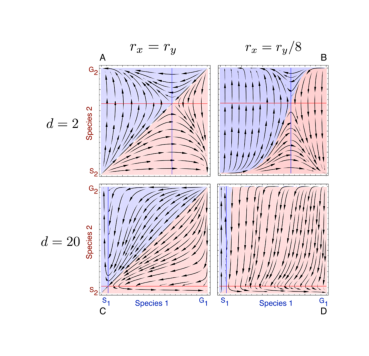
\includegraphics[width=\linewidth]{compare.eps}
\end{center}
\caption{
The composition of both species can range from all selfish $(S)$ to all generous $(G)$. 
If the other species is sufficiently generous, selfish behavior is favored in both species.
However, if the other species is selfish, generous behavior is advantageous.  
This is captured by the snowdrift game discussed in the text.
For equal evolutionary rates, $r_x=r_y$, the domains of attraction for the two outcomes $(S_1, G_2)$ and $(G_1, S_2)$
are of equal size (Panels A and C).
The colors illustrate the regions leading to the outcomes favorable to species $1$ (blue shaded area leading to $(S_1, G_2)$) 
and species $2$ (red shaded area leading to $(G_1, S_2)$).
For a two player game, $d=2$, and $r_x=r_y/8$, the basin of attraction favorable to the slower evolving species $1$ grows substantially (Panel B) \citep{bergstrom:2003jf}.
For a twenty player game, $d=20$, the basins of attractions have identical size for equal evolutionary rates, but the position of the internal equilibrium is shifted (Panel C).
When species $1$ evolves slower than species $2$ in this situation, most of the initial conditions in the simplex lead to a solution which is unfavorable to species $1$.
Thus for 20 players instead of two, the Red King effect is reversed ($b=2$ and $c=1$).
\label{fig:compare}
}
\end{figure}

Note that for $d=2$, $M=1$, $b=2$, $c=1$ we recover the matrix used in \citep{bergstrom:2003jf}.
Even for these new fitness functions for multiplayer games, the dynamics are still given by the replicator equations \citep{hauert:2006fd,pacheco:2009aa,gokhale:2010pn}.
Also note that for two player games with $M=1$, there are four fixed points on the vertices of the state space and the one internal one given by $x = y = 2 (b-c)/(2 b - c) = \frac{2}{3}$.
The position of the interior fixed point is independent of the evolutionary rates.
For a $20$ player game, the basins of attractions are still of the same size, but the dynamics leading to the stable points on the vertices are completely different (Fig. \ref{fig:compare} Panel C, $r_x=r_y$).
The internal equilibrium has now shifted to $x = y = 0.063$.
As before, we introduce an asymmetry in the evolutionary rates as $r_x = r_y /8$.
Interestingly, we find that for a $20$ player game (Fig. \ref{fig:compare} Panel D, $r_x=r_y/8$) for the same asymmetric values of growth rates as in the two player case, most of the initial conditions in the simplex lead to a stable point where species $2$ is selfish and species $1$ is generous ($G_1$, $S_2$).
This  reverses the outlook which we got from $d=2$.
Everything else being the same, in the presence of multiple players, the Red King effect is not observed.

Next, we explore the exact process due to which the Red King effect vanishes.
The replicator solutions of the two species creates quadrants in the simplex.
Of these quadrants, the top right and the bottom left are of special interest as they contain the separatrix between the two basins of attraction.
Consider the top right quadrant.
Species $2$ is represented by the $y-axis$, hence a faster evolution by species $2$ results in most of the initial conditions leading to the outcome favorable for species $2$, i.e. $(G_1,S_2)$.
An exactly opposite scenario is taking place in the bottom left quadrant.
Hence in this quadrant as species $1$ is evolving at a slower pace than species $2$, most of the initial condition here lead to an outcome favoring species $1$, i.e. $(S_1, G_2)$.
As long as the internal equilibrium is on the diagonal the Red King effect depends on the sizes of these quadrants.
Changing the number of players alters the sizes of these two influential quadrants.
For example consider the case of the twenty player game.
The size of the bottom left quadrant is reduced to such an extent that almost the whole of the simplex leads to the outcome favorable for the faster evolving species.


Obviously, the bottom left and the top right quadrants have equal size when the internal equilibrium is at $x = y = 0.5$.
For a fixed $b$ and $c$ we cannot select any arbitrary number of players $d$ to obtain this equilibrium, as $d$ is not a continuous variable.
If the equilibrium is above $x = 0.5$, then a decrease in the evolutionary rate can be beneficial as demonstrated by the Red King effect. 
Conversely, if the equilibrium is below $x=0.5$, then an increase in the evolutionary rate might be favorable.
Hence the Red Queen dynamics would favour a species even in the mutualistic setting if the number of players is effective in positioning the equilibrium at $x<0.5$.

Interspecific relationships are exceedingly complex \citep{blaser:2007aa}.
It might be challenging to find the exact number of species interacting together to maintain the system \citep{doebeli:1998aa,bronstein:2002aa,bascompte:2006aa} and furthermore to find if the interactions are balanced.
Asymmetries have been considered in mutualistic species at the level of species or other properties of the system such as interactions \citep{noe:1991aa}, interaction lengths \citep{johnstone:2002aa} or growth rates \citep{bergstrom:2003jf}.
Asymmetry in the number of interacting partners has only been recently tackled \citep{wang:2011aa}.
Going back to the example of ants and larvae, a single larva is tended by multiple ants.
Thus while from each ants point of view this is a two player game, for the larva this would be a multi-player game.

\begin{figure}
\begin{center}
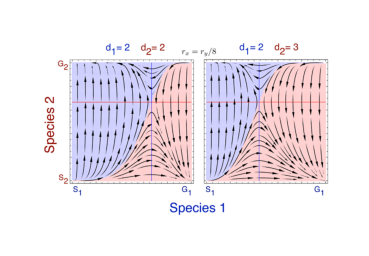
\includegraphics[width=\linewidth]{asymplandrate.eps}
\end{center}
\caption{
The Red King effect can be neutralized and/or even reversed if the number of players increases.
Here we show the scenario explored in \citep{bergstrom:2003jf} on the left panel;
a two player game ($d_1 = d_2 = 2$) with $r_x=r_y/8$.
Most of the points in the simplex lead towards the state favourable for species $1$, ($S_1,G_2$).
This changes when the number of players in species $2$ increases from $d_2=2$ to $d_2=3$,
i.e.\ now one individuals of species 2 interact with two individuals of species $1$. 
The vertical and horizontal lines denote the positions where the the change in the strategy frequency is zero for species $1$ and $2$ respectively.
The solution for species $1$ (vertical, blue line) moves towards smaller $x$, increasing the size of the top right quadrant.
For $d_1=2$ and $d_2=3$, it is given by $x = \frac{3 (2 b-c) - \sqrt{3 (4 b c - c^2)} }{2 (3 b -c)}$, whereas the 
the solution for species $2$ is still $ y = \frac{2(b-c)}{2 b - c}$ (see Appendix).  
Thus, the quadrant favoring the species with a faster evolutionary rate grows.
Since the number of players affects the size of these quadrants, it can eliminate or magnify the Red King effect.
}
\label{fig:counter}
\end{figure}

An interesting situation arises when we couple asymmetric number of players and asymmetric evolutionary rates. 
Instead of the single parameter $d$, now we have $d_1$ and $d_2$ as the number of players for the two species $1$ and $2$.
For symmetric evolutionary rates, if one species plays a more player game than the other species then there are more points in the simplex from where the selfish outcome is accessible.
For equal number of players, it depends on the sizes of the quadrants if a species should have a faster or slower rate of evolution to get the upper hand in the mutualistic relationship.
Hence, if a species is currently at a disadvantage, a modification of the number of players or the evolutionary rate can sometimes put it on equal footing with the other species. 
Due to asymmetric number of players the sizes of the basins of attraction depends not just on the sizes of the quadrants but the shape of the separatrix as well.
Thus, it is possible to counter the Red King effect by changing the number of interacting agents (Fig.\ \ref{fig:counter}).

Considering multi-player games provides a hitherto unexplored phenomenon in these kind of mutualism models.
When a species interacts with a number of individuals of another species in a mutualistic relationship, it is possible that a certain quorum needs to be fulfilled.
Client fish have been shown to choose cleaning stations with two cleaners over solitary cleaners \citep{bshary:2002aa}.
A certain number of ants are required to save a myrmecophilous caterpillar from it's predator.
It has been shown that the amount of larval secretions is correlated to the number of attending ants \citep{axen:1998aa}.

Until now, we have considered this threshold to be one ($M=1$).
To begin with the simplest multiplayer case, we consider
a symmetric three player game with different thresholds in either species to start off the benefits of mutualistic relations (say for species $1$ the threshold is $M_1$ and similarly for species $2$ is $M_2$ where in general $M_i$ can range from $1$ to $d_i$).

The payoff matrices become asymmetric due to the different thresholds for the two species.
Here, it matters which dynamics we are studying, the usual replicator dynamics or the modified replicator equations (Figs.\ \ref{fig:thresholdsrep} and \ref{fig:thresholdsmodrep}) (see Appendix) as they can result in different sizes of the basins of attraction.
We can also change the nature of the game from coexistence to coordination by manipulating these thresholds \citep{souza:2009aa} and hence intuitively translate between different social dilemmas when studying multi-player games.


\begin{figure}[h]
\begin{center}

\includegraphics[width=\linewidth]{standardreplicator.eps}
\end{center}
\caption{
A three player game with asymmetric thresholds, but $r_x=r_y$.
Species $1$ and species $2$ are both playing a three player game.
For species $1$, it is enough if one individual is \textit{``Generous"} to produce the benefit ($M_1 = 1$).
For species $2$, however, the minimum number of \textit{``Generous"} players required to produce any benefit 
strongly affects the replicator dynamics. 
For $M_2=M_1=1$, we observe the basins of attraction discussed above. 
The manifolds for the saddle point plotted forward in time (dashed green lines) and backward in time (solid green lines) can be used to define the basins of attraction.
For $M_2=2$, we observe a region with closed orbits in the interior (white background), almost all initial conditions outside this region lead to ($G_1,S_2$). 
For $M_2=3$, we observe closed orbits in almost the whole simplex. 
To avoid negative payoffs and to facilitate the comparison with other dynamics, we have added a background fitness of  $1.0$ to all payoffs, but this does not alter the dynamics here.
}
\label{fig:thresholdsrep}
\end{figure}

\section*{Discussion}

Development of a game theoretical approach for mutualism requires a different outlook from the social dilemmas field \citep{bshary:2004aa}.
In a mutualistic framework, it is best for the two species to cooperate with each other.
We do not ask the question how these mutualisms arise. 
Rather when they do, what is the best strategy to contribute towards the common benefit \citep{bshary:2003bo,bowles:2003uw}?
It would be possible to include the interactions between the individuals of the same species, as has been explored experimentally recently \citep{wang:2011aa}.
But then, we would be shifting our focus from the problem of interspecific mutualism to intraspecific cooperation \citep{bshary:2008aa}.
Here, we have focused on the interspecific interactions, where the interacting partners are always picked from the other species \citep{schuster:1981aa}.
Bergstrom and Lachmann have shown that in such a mutualistic scenario, the species which evolves slower can get away with being selfish and force the other species to make a generous contribution.
They termed this as the Red King effect.
If we include multiple players then the Red King effect is much more complex.

For simplicity, usually pairwise interactions are assumed in game theoretical arguments.
For modeling collective phenomenon, multiplayer games may be necessary.
The exact number of players is a matter of choice, though.
Group size distributions give us an idea about the mean group size of a species.
Instead of using pairwise interactions or an arbitrary number of individuals to form a group, we could use the mean group sizes as the number of interacting individuals.
Group size is known to be of importance in mutualisms \citep{wilson:1983an}.
As we have seen here, it can be a influential factor in deciding how the benefits are shared.
Countering the Red King or enhancing its effect is possible by altering the group size.
Hence can the group size itself be an evolving strategy?
The study of group size distributions has been tackled theoretically \citep{krause:2002bo,hauert:2002te, niwa:2003gs,hauert:2006ha, hauert:2008bb,veelen:2010gc,sumpter:2010bo,braennstroem:2011mb,pena:2011aa} and empirically in various species ranging from house sparrows to humans \citep{zipf:1949sg,krause:2002bo,sumpter:2010bo,griesser:2011po}.
In our example of ants and butterfly larvae, it has been observed that a larva was most successful in getting more ant attendants in a group of four larvae \citep{pierce:1987aa}.
It would be interesting to see if the distributions in mutualistic species peak at the group size which is the best response to their symbiont partners choices.
Future work would also involve including intraspecific interactions and how they might affect interspecific relationships (as in \citet{bshary:2008aa}).
It has been shown in \cite{axen:1998aa} that the amount of larval secretions is also influenced by the quality of the other larvae in the group.
Another method of introducing asymmetry is to have different payoff tables for the two species (i.e. different benefits and costs for the two species).
Also we have just considered two strategies per species.
Asymmetric number of strategies can induce further asymmetries in the interaction \citep{schuster:1981aa}.
The intricacies of multiplayer games lend themselves to study such systems, but they also show that mutualisitc interactions may be far more complex than often envisioned.
Applying multiplayer game theory to mutualism unravels this dynamics between species and can be used to understand the complexity of these non-linear systems.


\section*{Acknowledgements} 
We thank Christian Hilbe, Aniek Ivens, Martin Kalbe, Michael Lachmann and Istv\`an Scheuring  for helpful discussions and suggestions. Financial support from the Emmy-Noether program of the DFG and from the Max Planck Society is gratefully acknowledged.

\begin{thebibliography}{58}
\providecommand{\natexlab}[1]{#1}
\providecommand{\url}[1]{\texttt{#1}}
\providecommand{\urlprefix}{URL }

\bibitem[{Abel(1824)}]{abel:1824aa}
Abel, N.~H., 1824.
\newblock M\'emoire sur les \'equations alg\'ebriques, o\`u l'on d\'emontre
  l'impossibilit\'e de la r\'esolution de l'\'equation g\'en\'erale du
  cinqui\'eme degr\'e.
\newblock Abel's Ouvres Pp. 28--33.

\bibitem[{Ak{\c c}ay and Roughgarden(2007)}]{akcay:2007aa}
Ak{\c c}ay, E. and J.~Roughgarden, 2007.
\newblock Negotiation of mutualism: rhizobia and legumes.
\newblock Proc. R. Soc. B 274:25--32.

\bibitem[{Aristotle(350 B.C.E.)}]{aristotle:350bc}
Aristotle, 350 B.C.E.
\newblock The History of Animals (Translated by: D'Arcy Wentworth Thompson).

\bibitem[{Ax{\'e}n and Pierce(1998)}]{axen:1998aa}
Ax{\'e}n, A.~H. and N.~E. Pierce, 1998.
\newblock Aggregation as a cost-reducing strategy for lycaenid larvae.
\newblock Behavioral Ecology 9:109--115.

\bibitem[{Bascompte et~al.(2006)Bascompte, Jordano, and
  Olesen}]{bascompte:2006aa}
Bascompte, J., P.~Jordano, and J.~M. Olesen, 2006.
\newblock {Asymmetric Coevolutionary Networks Facilitate Biodiversity
  Maintenance}.
\newblock Science 312:431--433.

\bibitem[{Bergstrom and Lachmann(2003)}]{bergstrom:2003jf}
Bergstrom, C.~T. and M.~Lachmann, 2003.
\newblock The red king effect: When the slowest runner wins the coevolutionary
  race.
\newblock Proc. Natl. Acad. Sci. USA 100:593--598.

\bibitem[{Blaser and Kirschner(2007)}]{blaser:2007aa}
Blaser, M.~J. and D.~Kirschner, 2007.
\newblock The equilibria that allow bacterial persistance in human hosts.
\newblock Nature 449:843--849.

\bibitem[{Boucher(1985)}]{boucher:1985aa}
Boucher, D.~H., 1985.
\newblock The idea of mutualism, past and future.
\newblock Pp. 1--28, \emph{in} D.~H. Boucher, ed. The Biology of Mutualism.
  Oxford University Press, New York.

\bibitem[{Bowles and Gintis(2003)}]{bowles:2003uw}
Bowles, S. and H.~Gintis, 2003.
\newblock The origins of human cooperation.
\newblock \emph{in} P.~Hammerstein, ed. The Genetic and Cultural Origins of
  Cooperation. MIT Press, Cambridge.
\newblock To appear in.

\bibitem[{Br{\"a}nnstr{\"o}m et~al.(2011)Br{\"a}nnstr{\"o}m, Gross, Blasius,
  and Dieckmann}]{braennstroem:2011mb}
Br{\"a}nnstr{\"o}m, {\AA}., T.~Gross, B.~Blasius, and U.~Dieckmann, 2011.
\newblock Consequences of fluctuating group size for the evolution of
  cooperation.
\newblock J. Math. Biol. 63:263--281.

\bibitem[{Bronstein(1994)}]{bronstein:1994aa}
Bronstein, J.~L., 1994.
\newblock Our current understanding of mutualism.
\newblock The Quarterly Review of Biology 69:31--51.

\bibitem[{Bronstein(2003)}]{bronstein:2003bo}
---{}---{}---, 2003.
\newblock Exploitation within mutualistic interactions.
\newblock \emph{in} P.~Hammerstein, ed. Genetic and Cultural Evolution of
  Cooperation. MIT Press.

\bibitem[{Bronstein and Barbosa(2002)}]{bronstein:2002aa}
Bronstein, J.~L. and P.~Barbosa, 2002.
\newblock Multitrophic Level Interactions, chap. Multitrophic/multispecies
  mutualistic interactions: the role of non-mutualists in shaping and mediating
  mutualisms.
\newblock Cambridge University Press.

\bibitem[{Bshary et~al.(2008)Bshary, Grutter, Willener, and
  Leimar}]{bshary:2008aa}
Bshary, R., A.~S. Grutter, A.~S.~T. Willener, and O.~Leimar, 2008.
\newblock Pairs of cooperating cleaner fish provide better service quality than
  singletons.
\newblock Nature 455:964--967.

\bibitem[{Bshary and Sch{\"a}ffer(2002)}]{bshary:2002aa}
Bshary, R. and D.~Sch{\"a}ffer, 2002.
\newblock Choosy reef fish select cleaner fish that provide high-quality
  service.
\newblock Animal Behaviour 63:557--564.

\bibitem[{Bshary and Bronstein(2004)}]{bshary:2004aa}
Bshary, R.~S. and J.~L. Bronstein, 2004.
\newblock Game structures in mutualisms: what can the evidence tell us about
  the kinds of models we need?
\newblock Advances in the Study of Behavior 34:59--104.

\bibitem[{Bshary and No\"{e}(2003)}]{bshary:2003bo}
Bshary, R.~S. and R.~No\"{e}, 2003.
\newblock Biological markets: the ubiquitous influence of partner choice on the
  dynamics of cleaner fish-client reef fish interactions.
\newblock Pp. 167--184, \emph{in} P.~Hammerstein, ed. Genetic and Cultural
  Evolution of Cooperation. MIT Press.

\bibitem[{Damore and Gore(2011)}]{damore:2011ev}
Damore, J.~A. and J.~Gore, 2011.
\newblock A slowly evolving host moves first in symbiotic interactions.
\newblock Evolution 65:2391--2398.

\bibitem[{Doebeli and Knowlton(1998)}]{doebeli:1998aa}
Doebeli, M. and N.~Knowlton, 1998.
\newblock The evolution of interspecific mutualisms.
\newblock Proc. Natl. Acad. Sci. USA 95:8676--8680.

\bibitem[{Gokhale and Traulsen(2010)}]{gokhale:2010pn}
Gokhale, C.~S. and A.~Traulsen, 2010.
\newblock Evolutionary games in the multiverse.
\newblock Proc. Natl. Acad. Sci. USA 107:5500--5504.

\bibitem[{Griesser et~al.(2011)Griesser, Ma, Webber, Bowgen, and
  Sumpter}]{griesser:2011po}
Griesser, M., Q.~Ma, S.~Webber, K.~Bowgen, and D.~J.~T. Sumpter, 2011.
\newblock Understanding animal group-size distributions.
\newblock PLoS ONE 6:e23438.

\bibitem[{Hauert et~al.(2002)Hauert, De~Monte, Hofbauer, and
  Sigmund}]{hauert:2002te}
Hauert, C., S.~De~Monte, J.~Hofbauer, and K.~Sigmund, 2002.
\newblock Volunteering as red queen mechanism for cooperation in public goods
  games.
\newblock Science 296:1129--1132.

\bibitem[{Hauert et~al.(2006{\natexlab{a}})Hauert, Holmes, and
  Doebeli}]{hauert:2006ha}
Hauert, C., M.~Holmes, and M.~Doebeli, 2006{\natexlab{a}}.
\newblock Evolutionary games and population dynamics:maintenance of cooperation
  in public goods games.
\newblock Proc. Roy. Soc. Lond. B 273:2565--2570.

\bibitem[{Hauert et~al.(2006{\natexlab{b}})Hauert, Michor, Nowak, and
  Doebeli}]{hauert:2006fd}
Hauert, C., F.~Michor, M.~A. Nowak, and M.~Doebeli, 2006{\natexlab{b}}.
\newblock Synergy and discounting of cooperation in social dilemmas.
\newblock J. Theor. Biol. 239:195--202.

\bibitem[{Hauert et~al.(2008)Hauert, Traulsen, Brandt, Nowak, and
  Sigmund}]{hauert:2008bb}
Hauert, C., A.~Traulsen, H.~Brandt, M.~A. Nowak, and K.~Sigmund, 2008.
\newblock Public goods with punishment and abstaining in finite and infinite
  populations.
\newblock Biological Theory 3:114--122.

\bibitem[{Hill and Pierce(1989)}]{hill:1989aa}
Hill, C.~J. and N.~E. Pierce, 1989.
\newblock The effect of adult diet on the biology of butterflies 1. the common
  imperial blue, \textit{Jalmenus evagoras}.
\newblock Oecologia 81:249--257.

\bibitem[{Hinton(1951)}]{hinton:1951aa}
Hinton, H.~E., 1951.
\newblock Myrmecophilous lycaenidae and other lepidoptera - a summary.
\newblock Proc. Trans. S. London Entomol. Nat. Hist. Soc. 1949-50:111--175.

\bibitem[{Hoeksema and Kummel(2003)}]{hoeksema:2003aa}
Hoeksema, J.~D. and M.~Kummel, 2003.
\newblock Ecological persistence of the plant-mycorrhizal mutualism: A
  hypothesis from species coexistence theory.
\newblock The American Naturalist 162:S40--S50.

\bibitem[{Hofbauer(1996)}]{hofbauer:1996mm}
Hofbauer, J., 1996.
\newblock Evolutionary dynamics for bimatrix games: A {H}amiltonian system?
\newblock J. Math. Biol. 34:675--688.

\bibitem[{Hofbauer and Sigmund(1998)}]{hofbauer:1998mm}
Hofbauer, J. and K.~Sigmund, 1998.
\newblock Evolutionary Games and Population Dynamics.
\newblock Cambridge University Press, Cambridge, UK.

\bibitem[{Hofbauer and Sigmund(2003)}]{hofbauer:2003mm}
---{}---{}---, 2003.
\newblock Evolutionary game dynamics.
\newblock Bull. Am. Math. Soc. 40:479--519.

\bibitem[{H{\"o}lldobler and Wilson(1990)}]{holldobler:1990an}
H{\"o}lldobler, B. and E.~O. Wilson, 1990.
\newblock The Ants.
\newblock Belknap Press.

\bibitem[{Johnstone and Bshary(2002)}]{johnstone:2002aa}
Johnstone, R.~A. and R.~Bshary, 2002.
\newblock From parasitism to mutualism: partner control in asymmetric
  interactions.
\newblock Ecology Letters 5:634--639.

\bibitem[{Kiers et~al.(2003)Kiers, Rosseau, West, and Denison}]{kiers:2003aa}
Kiers, E.~T., R.~A. Rosseau, S.~A. West, and R.~F. Denison, 2003.
\newblock Host sanctions and the legume-rhizobium mutualism.
\newblock Nature 425.

\bibitem[{Krause and Ruxton(2002)}]{krause:2002bo}
Krause, J. and G.~Ruxton, 2002.
\newblock Living in groups.
\newblock Oxford University Press.

\bibitem[{Mack and Rudgers(2008)}]{mack:2008aa}
Mack, K. M.~L. and J.~A. Rudgers, 2008.
\newblock Balancing multiple mutualists: asymmetric interactions among plants,
  arbuscular mycorrhizal fungi, and fungal endophytes.
\newblock Oikos 117:310--320.

\bibitem[{Maynard~Smith(1982)}]{maynard-smith:1982to}
Maynard~Smith, J., 1982.
\newblock Evolution and the Theory of Games.
\newblock Cambridge University Press, Cambridge.

\bibitem[{Niwa(2003)}]{niwa:2003gs}
Niwa, H.-S., 2003.
\newblock Power-law versus exponential distributions of animal group sizes.
\newblock Journal of theoretical Biology 224:451--457.

\bibitem[{No{\"e}(2001)}]{noe:2001aa}
No{\"e}, R., 2001.
\newblock Biological markets: partner choice as the driving force behind the
  evolution of mutualisms.
\newblock \emph{in} R.~No{\"e}, J.~A. van Hooff, and P.~Hammerstein, eds.
  Economics in Nature: Social Dilemmas, Mate Choice and Biological Markets.
  Cambridge University Press.

\bibitem[{No{\"e} et~al.(1991)No{\"e}, van Schaik, and van Hooff}]{noe:1991aa}
No{\"e}, R., C.~P. van Schaik, and J.~A. R. A.~M. van Hooff, 1991.
\newblock The markert effect: an explanation for pay-off asymmetries among
  collaborating animals.
\newblock Ethology 87:97--118.

\bibitem[{Pacheco et~al.(2009)Pacheco, Santos, Souza, and
  Skyrms}]{pacheco:2009aa}
Pacheco, J.~M., F.~C. Santos, M.~O. Souza, and B.~Skyrms, 2009.
\newblock {Evolutionary dynamics of collective action in N-person stag hunt
  dilemmas.}
\newblock Proc. R. Soc. B 276:315--321.

\bibitem[{Pe{\~n}a(2011)}]{pena:2011aa}
Pe{\~n}a, J., 2011.
\newblock Group size diversity in public goods games.
\newblock Evolution Accepted Article.

\bibitem[{Pierce et~al.(2002)Pierce, Braby, Heath, Lohman, Mathew, Rand, and
  Travassos}]{pierce:2002aa}
Pierce, N.~E., M.~F. Braby, A.~Heath, D.~J. Lohman, J.~Mathew, D.~B. Rand, and
  M.~A. Travassos, 2002.
\newblock {The Ecology and Evolution of Ant Association in the Lycaenidae
  (Lepidoptera)}.
\newblock Annu. Rev. Entomol 47:733--770.

\bibitem[{Pierce et~al.(1987)Pierce, Kitching, Buckley, Taylor, and
  Benbow}]{pierce:1987aa}
Pierce, N.~E., R.~L. Kitching, R.~C. Buckley, M.~F.~J. Taylor, and K.~F.
  Benbow, 1987.
\newblock The costs and benefits of cooperation between the australian lycaenid
  butterfly, \textit{Jalmenus evagoras} and its attendant ants.
\newblock Behavioral Ecology and Sociobiology 21:237--248.

\bibitem[{Poulin and Vickery(1995)}]{poulin:1995aa}
Poulin, R. and W.~L. Vickery, 1995.
\newblock Cleaning symbiosis as an evolutionary game: to cheat or not to cheat?
\newblock J Theor Biol 175:63--70.

\bibitem[{Schuster et~al.(1981)Schuster, Sigmund, Hofbauer, and
  Wolff}]{schuster:1981aa}
Schuster, P., K.~Sigmund, J.~Hofbauer, and R.~Wolff, 1981.
\newblock Selfregulation in behaviour in animal societies ii. games between two
  populations without selfinteractions.
\newblock Biological Cybernetics 40:9--15.

\bibitem[{Souza et~al.(2009)Souza, Pacheco, and Santos}]{souza:2009aa}
Souza, M.~O., J.~M. Pacheco, and F.~C. Santos, 2009.
\newblock {Evolution of cooperation under N-person snowdrift games}.
\newblock J. Theor. Biol. 260:581--588.

\bibitem[{Stadler and Dixon(2008)}]{stadler:2008bo}
Stadler, B. and A.~F.~G. Dixon, 2008.
\newblock Mutualism: Ants and their Insect partners.
\newblock Cambridge University Press.

\bibitem[{Stewart(2004)}]{stewart:2004aa}
Stewart, I., 2004.
\newblock Galois theory. Third Edition.
\newblock Chapman \& Hall/CRC.

\bibitem[{Sumpter(2010)}]{sumpter:2010bo}
Sumpter, D. J.~T., 2010.
\newblock Collective animal behavior.
\newblock Princeton University Press.

\bibitem[{Taylor and Jonker(1978)}]{taylor:1978wv}
Taylor, P.~D. and L.~Jonker, 1978.
\newblock Evolutionary stable strategies and game dynamics.
\newblock Math. Biosci. 40:145--156.

\bibitem[{Trivers(1971)}]{trivers:1971hp}
Trivers, R.~L., 1971.
\newblock The evolution of reciprocal altruism.
\newblock The Quarterly Review of Biology 46:35--57.

\bibitem[{van Valen(1973)}]{vanVaalen:1973aa}
van Valen, L., 1973.
\newblock A new evolutionary law.
\newblock Evolutionary Theory 1:1--30.

\bibitem[{van Veelen et~al.(2010)van Veelen, Garcia, and
  Aviles}]{veelen:2010gc}
van Veelen, M., J.~Garcia, and L.~Aviles, 2010.
\newblock It takes grouping and cooperation to get sociality.
\newblock Journal of theoretical Biology 264:1240--1253.

\bibitem[{Wang et~al.(2011)Wang, Sun, Zheng, Shi, and Zhu}]{wang:2011aa}
Wang, R.-W., B.-F. Sun, Q.~Zheng, L.~Shi, and L.~Zhu, 2011.
\newblock Asymmetric interaction and indeterminate fitness correlation between
  cooperative partners in the fig -fig wasp mutualism.
\newblock Journal of The Royal Society Interface .

\bibitem[{Weibull(1995)}]{weibull:1995hp}
Weibull, J., 1995.
\newblock Evolutionary Game Theory.
\newblock MIT Press, Cambridge, MA.

\bibitem[{Wilson(1983)}]{wilson:1983an}
Wilson, D.~S., 1983.
\newblock The effect of population structure on the evolution of mutualism: A
  field test involving burying beetles and their phoretic mites.
\newblock The American Naturalist 121:851--870.

\bibitem[{Zipf(1949)}]{zipf:1949sg}
Zipf, G.~K., 1949.
\newblock Human Behaviour and the Principle of Least Effort.
\newblock Addison-Wesley, Cambridge.

\end{thebibliography}



\newpage


\section*{Appendix}
\section*{Average payoffs in the bimatrix game}
\label{appA}
\subsection*{Two player setting}

We can write down the payoff matrices for the two species separately  denoted by $A$ and $B$ as,
\begin{tabular}{cccccc}
& & & \multicolumn{2}{c}{Species 2} &\\
& & & $G_2$ & $S_2$ &\\
\multirow{2}{*}{$A$ = Species 1}& $G_1$
& \multirow{2}{*}{$\bigg($} & $a_{G_1,G_2}$ & $a_{G_1,S_2}$ & \multirow{2}{*}{$\bigg)$}\\
& $S_1$ & & $a_{S_1,G_2}$ & $a_{S_1,S_2}$ &
\end{tabular}
\begin{tabular}{cccccc}
& & & \multicolumn{2}{c}{Species 1} &\\
& & & $G_1$ & $S_1$ &\\
\multirow{2}{*}{B = Species 2}& $G_2$
& \multirow{2}{*}{$\bigg($} & $a_{G_2,G_1}$ & $a_{G_2,S_1}$ & \multirow{2}{*}{$\bigg)$}\\
& $S_2$ & & $a_{S_2,G_1}$ & $a_{S_2,S_1}$ &\ \ .
\end{tabular}
The frequency of the players playing strategy \textit{``Generous"} in species $1$ is given by $x$ and that in species $2$ by $y$.
As the population size is kept constant the reciprocal frequencies of the players playing \textit{``Selfish"} strategy are $1-x$ and $1-y$ in the two species respectively.

\subsection*{Multiplayer setting}
\label{appB}

For a multiplayer snowdrift game, the payoff entries are defined as \citep{souza:2009aa},
\begin{align}
\Pi_{S_1} (k) & = \begin{cases} b & \textrm{if } k \geq M \\ 0 & \textrm{if } k < M \end{cases}
\\
\Pi_{G_1} (k) & = \begin{cases} b-\frac{c}{k} & \textrm{if } k \geq M \\  -\frac{c}{M} & \textrm{if } k < M \end{cases}
\end{align}
%
The selfish players get the benefit $b$ if the number of generous individuals in both species combined, $k$, is greater than or equal to the threshold $M$.
For the generous individuals, their effort is subtracted from the payoffs.
The effort is shared if the quorum size is met ($\frac{c}{M}$), but happens in vain for $k<M$. 
The fitnesses of the two strategies in species $1$ are given by,
%
\begin{align}
f_{G_1} (y) &= \sum_{k=0}^{d-1} \binom{d-1}{k}y^k (1-y)^{d-1-k} \Pi_{G_1}(k+1) \\
f_{S_1} (y) &= \sum_{k=0}^{d-1} \binom{d-1}{k}y^k (1-y)^{d-1-k} \Pi_{S_1}(k).
\label{fiteqs}
\end{align}
%
Following the same procedure for the two strategies in species $2$ leads to the average fitness
%
\begin{align}
\bar{f}_1 (x,y) &= x f_{G_1} (y)+(1-x) f_ {S_1}(y)\\
\bar{f}_2 (x,y) &= y f_{G_2} (x)+(1-y) f_{S_2}(x).
\label{avgfiteqs}
\end{align}
%

\section*{Dynamics in asymmetric conditions}

We have addressed two kinds of asymmetries in the game, the number of player and the thresholds in the two species.
We denote the number of players for species $1$ and species $2$ as $d_1$ and $d_2$, respectively, as in Fig.\ \ref{fig:counter}.
That is if species $2$ is playing a $d_2$ player game it means that one player from species $2$ interacts with $d_2-1$ players of species $1$.
For an asymmetry in the thresholds we use the two parameters $M_1\geq1$ and $M_2\geq1$ for the two species, respectively.

For asymmetric bimatrix games, there is a difference in the dynamics between the standard replicator dynamics and the 
alternative dynamics put forward by Maynard-Smith \citep{maynard-smith:1982to}.
For this dynamics, the average fitness of each species appears as a denominator,
\begin{align}
\dot{x} &= r_x x \left(f_{G_1}(y) -  \bar{f}_1(x,y) \right)/\bar{f}_1(x,y) \nonumber \\
\dot{y} &= r_y y \left(f_{G_2}(x) -  \bar{f}_2(x,y) \right)/\bar{f}_2(x,y).
\label{eq:repeqs}
\end{align}
In our asymmetric bimatrix game, the fixed point stability is affected by the choice of the dynamics, in contrast to the case of symmetric games. 
In Fig.\ \ref{fig:thresholdsmodrep}, we illustrate that the dynamics is different between the usual 
replicator dynamics and Eqs. \ref{eq:repeqs}

For $d_1=d_2 \geq 5$, the exact coordinates of the fixed point must be computed numerically \citep{abel:1824aa,stewart:2004aa}.

\begin{figure}
\begin{center}

\includegraphics[width=\linewidth]{modifiedrepdyn.eps}
\end{center}
\caption{
For the same parameters as in Fig.\ \ref{fig:thresholdsrep}, the modified replicator dynamics given by Eqs.\ \ref{eq:repeqs} leads to a different dynamics.
For $M_1=M_2=1$ (left), the dynamics is the same as for the standard replicator dynamics. 
For $M_2=2$ (middle) and $M_2=3$ (right), the formerly neutrally stable fixed point in the interior becomes a stable focus. 
Moreover, for $M_2=2$, the basin of attraction of $(G_1,S_2)$ becomes much larger with the modified replicator dynamics. 
Again, we have added a background fitness of $1.0$ to all the payoff entries so that all payoffs are positive.
}
\label{fig:thresholdsmodrep}
\end{figure}


\end{document}